\section{Performance Evaluation}
\label{sec:evaluation}
In this section, we evaluate the performance of the proposed low-complexity solution framework by numerical simulations.
We first elaborate our experiment setup in section \ref{subsec:basic}, and the evaluation results compared with other benchmarks show that .
Then we \fixit{do what} to apply the sensitivity study on the robustness of our proposed framework.

\subsection{Performance Analysis}
\label{subsec:basic}
\textbf{System Parameters Setup:}
\fixit{
    In the simulation, there are 5 APs, 3 ES and 10 type of jobs in the system.
}
We implement the system in a small scale setting where fully-accessible APs and edge servers are considered.
specifically, there are $K=5$ APs, $M=3$ edge servers, and $J=5$ type of jobs in the system corresponding to the manipulated data trace.
Each time slot is taken as $\tau = 0.05$ i.e. 50ms, and the broadcast interval is taken as $20$ time slots, i.e. $1$ second.
The maximum uploading time is set as $3$ times the broadcast interval, i.e. $\Xi = 3T$.
\fixit{
    The computation time of each job type at each edge server follows the uniform distribution.
}
The distributions of arrival rate, uploading time and processing time are generated randomly.
Each queue for VMs on edge server is set with maximum queue length $L_{max}=20$, i.e. there would be at most $100$ jobs on one edge server.
\fixit{
    We set small maximum queue length, in case to show that how job rejection affects the system.
}
% The arrival rate is taken as small probability with enough APs in the system, and correspondingly enough edge servers for the processing.
% Each queue on edge server with maximum 20 jobs because our algorithm is strong enough to predict the overflow to ensure a reliable system.

\begin{figure*}[ht!]
    \centering
    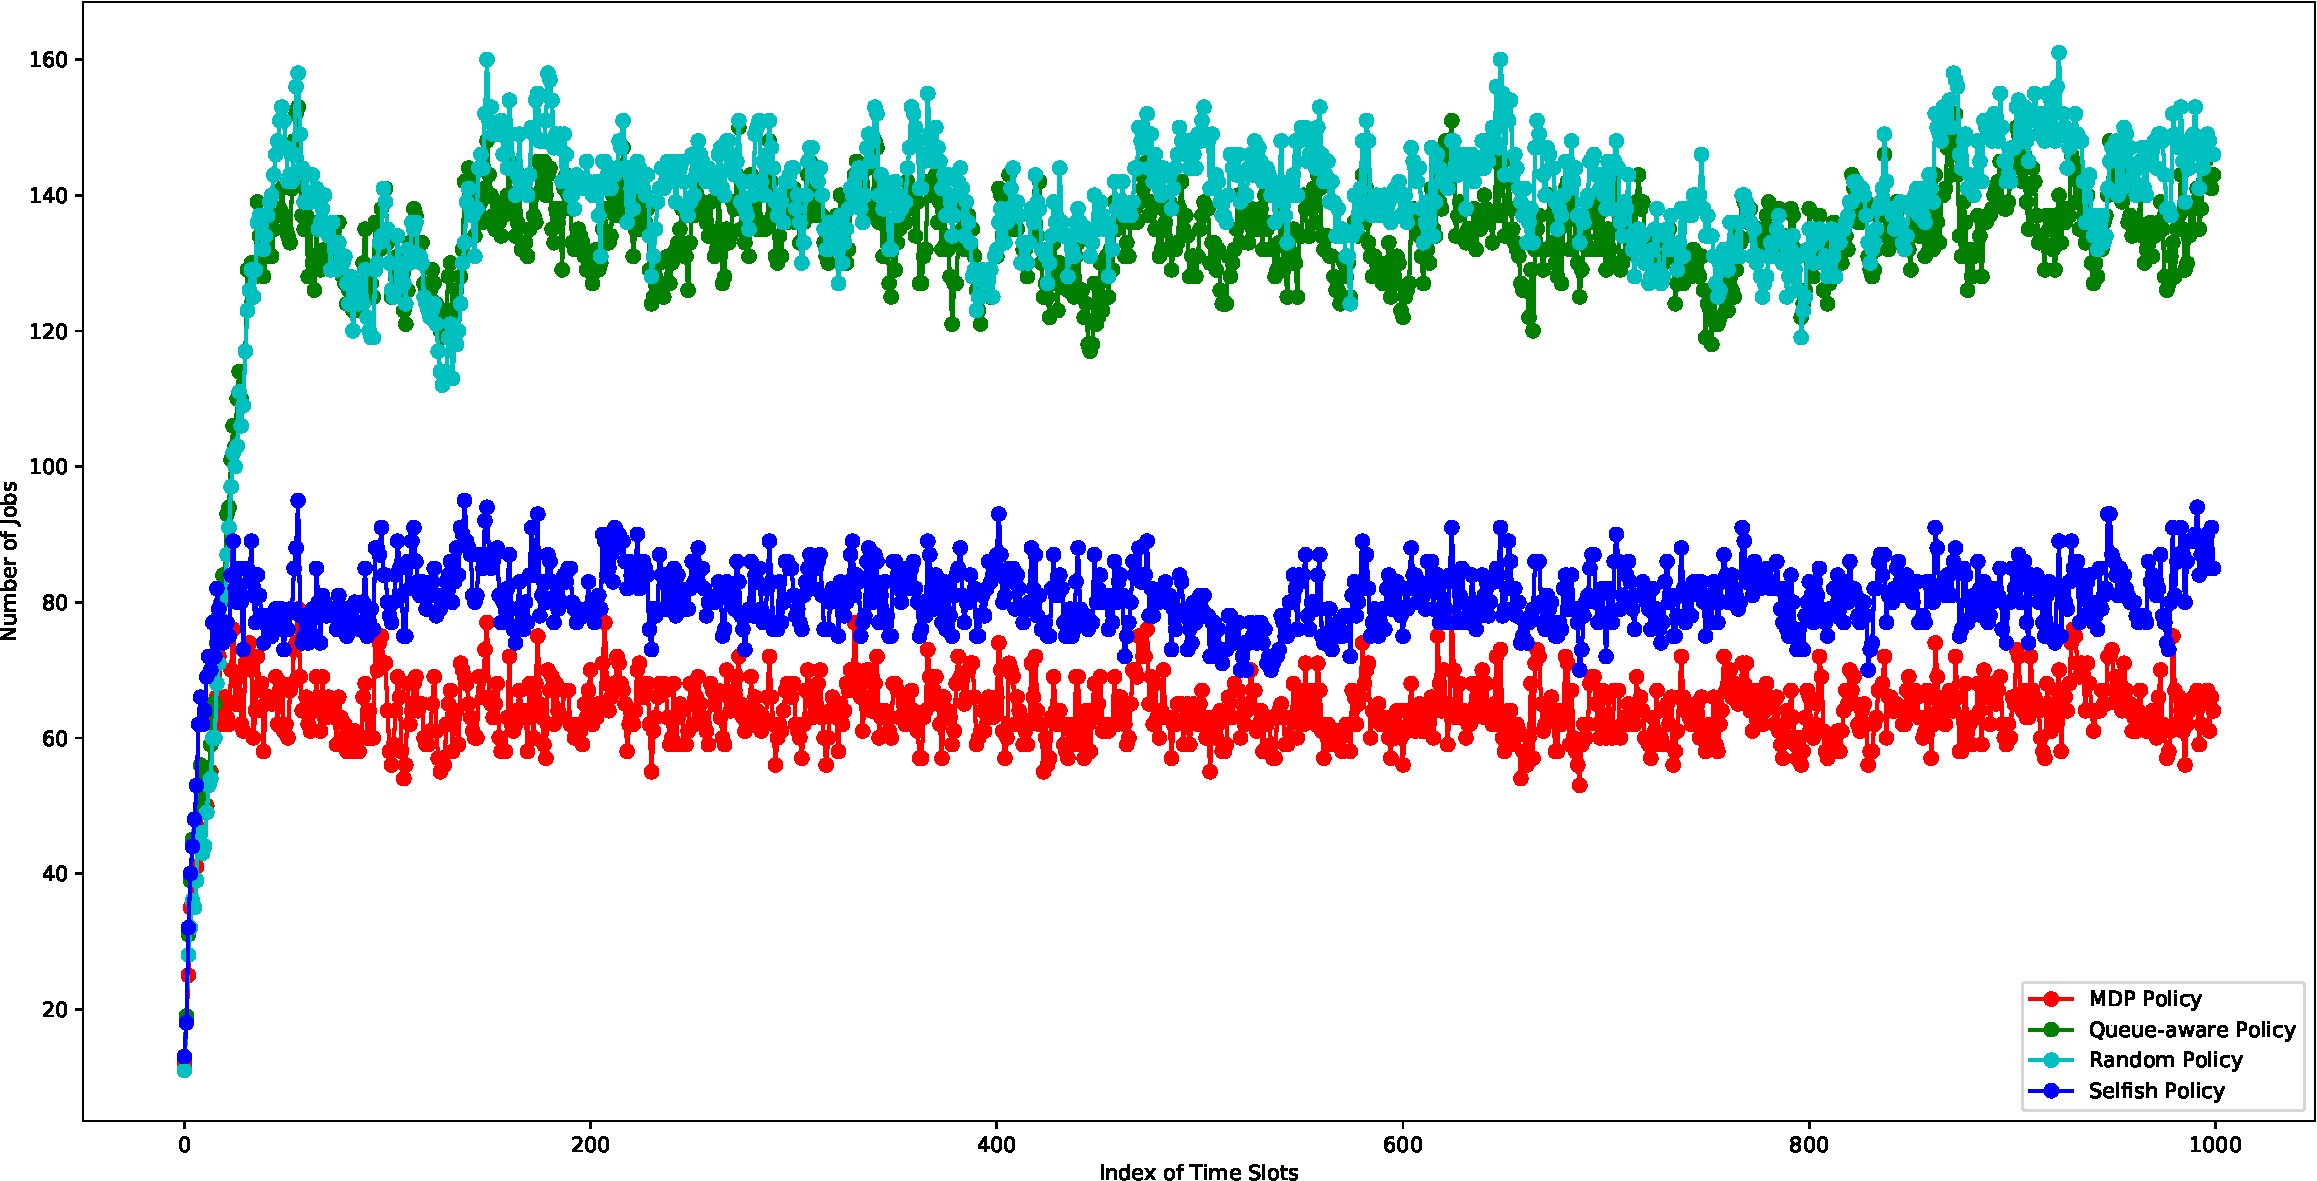
\includegraphics[width=0.80\textwidth]{48113-timeline-number.pdf}
    \caption{The illustration of number of jobs on all the APs and edge servers over time.}
    \label{fig:general_timeline}
\end{figure*}

%NOTE: Benchmark Elaboration
\fixit{The following four benchmark schemes are compared with the proposed scheduling scheme.}
\textbf{Benchmarks:}
We compare the proposed algorithm with other three heuristic algorithms which are listed as follows.
\begin{itemize}
    \item \textbf{Random Dispatching Policy}:
            for each job type, randomly choose the dispatching edge server in each time slot; 
    \item \textbf{Selfish Algorithm}:
            for each job type, always choose the edge server with the minimum expected uploading time, plus the expected processing time;
    \item \textbf{Queue-aware Selfish Algorithm}:
            for each job type, always choose the edge server with the minimum expected uploading time, plus the expected processing time and queueing time based on the observation of outdated queue states.
\end{itemize}
Specifically, we choose the \emph{Local Selfish Algorithm} which is state-invariant as the initial fixed policy for our proposed algorithm.
The explicit definition is given as follows.
\begin{policy}[Selfish Policy]
    \begin{align}
        \Baseline &\define \Brace{ \Pi_{k}\define\set{\pi_{k,j}|\forall j\in\jSpace} |\forall k\in\apSet },
    \end{align}
    where $\pi_{k,j} \define \arg\min_{m\in\esSet_{k}} u_{k,m,j} + c_{m,j}$.
\end{policy}

%NOTE: Basic Performance
Here we measure some basic metrics concerning in edge computing system, compared with different algorithms.
Average Cost v.s. Algorithms, Fig.\ref{fig:bar_plot}(a);
Average JCT (job completion time) v.s. Algorithms, Fig.\ref{fig:bar_plot}(b);
Average Departure Rate (throughput) v.s. Algorithms, Fig.\ref{fig:bar_plot}(c).

%-----------------------------------------------------------------------%
\begin{figure}[h]                                                       %
    \centering                                                          %
    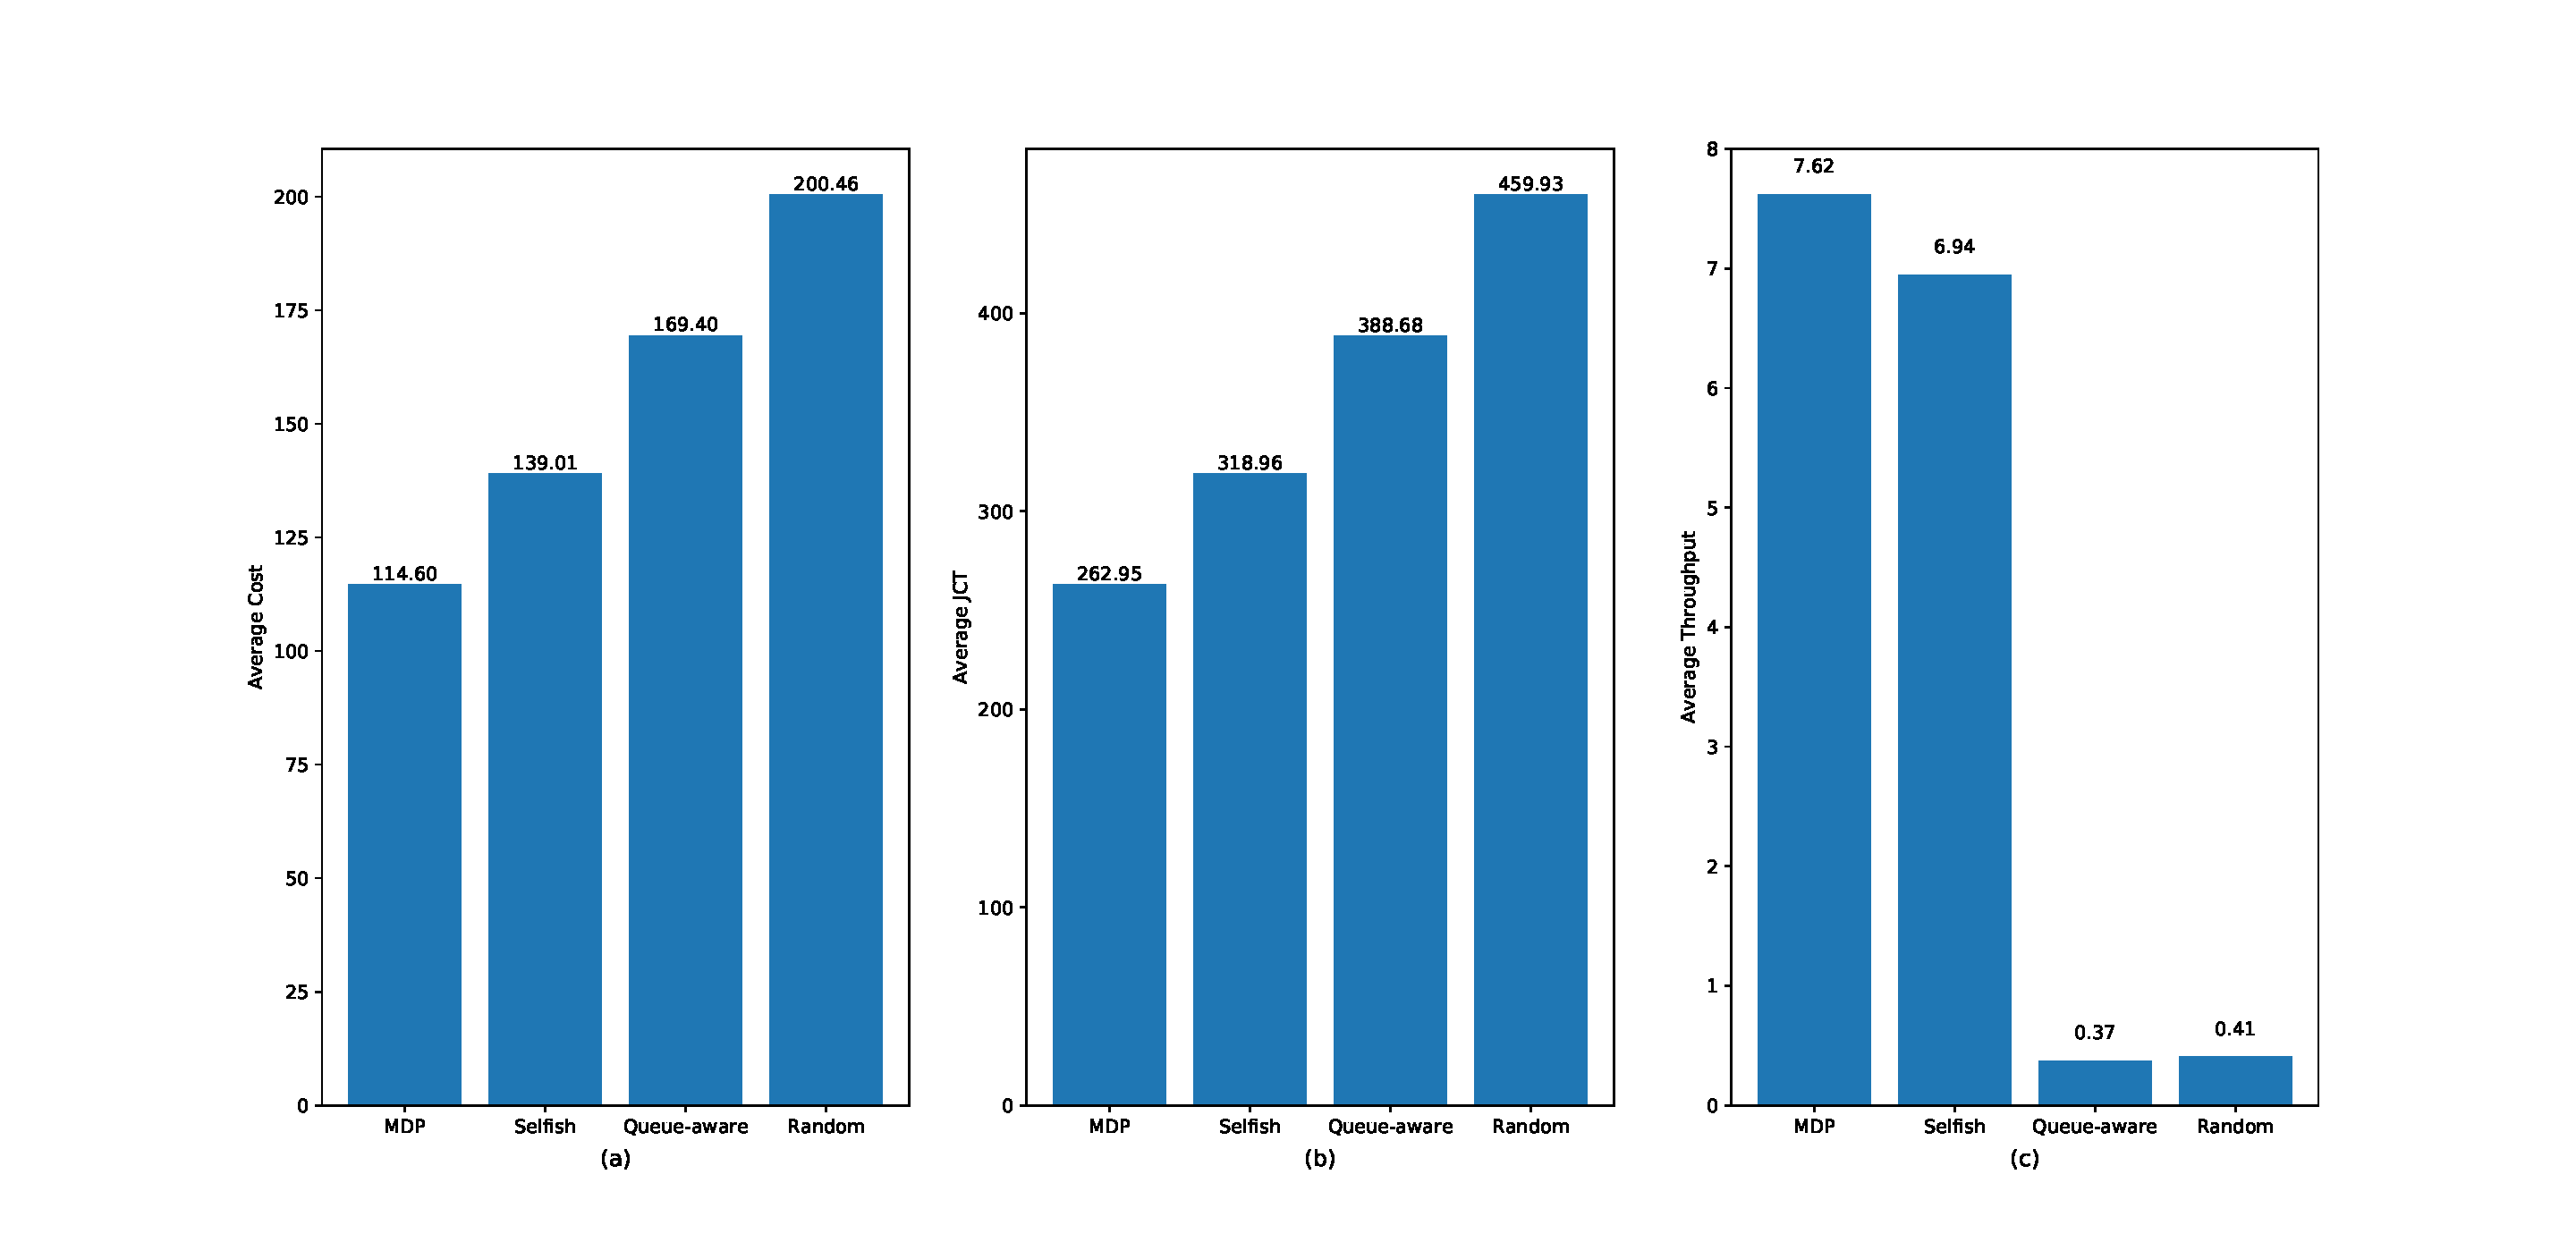
\includegraphics[width=0.45\textwidth]{48113-bar-graph.pdf}         %
    \caption{Basic performance comparison.}                             %
    \label{fig:bar_plot}                                                %
\end{figure}                                                            %
%-----------------------------------------------------------------------%

%NOTE: Insight Analysis
Specifically, 
our proposed algorithm is better than compared algorithms all the time;
CDF graph of Cost (with different benchmarks).
% \fixit{\blindtext}
% CDF graph of JCT (with different algorithms).
%----------------------------------------------------------------------------------------%
\subsection{Sensitivity Study}
\label{subsec:advance}
\blindtext

%FIXME: replace the graphs
%-----------------------------------------------------------------------------------------------%
\begin{figure*}[ht!]                                                                            %
    \centering                                                                                  %
    \begin{tabular}{ccc}                                                                        %
        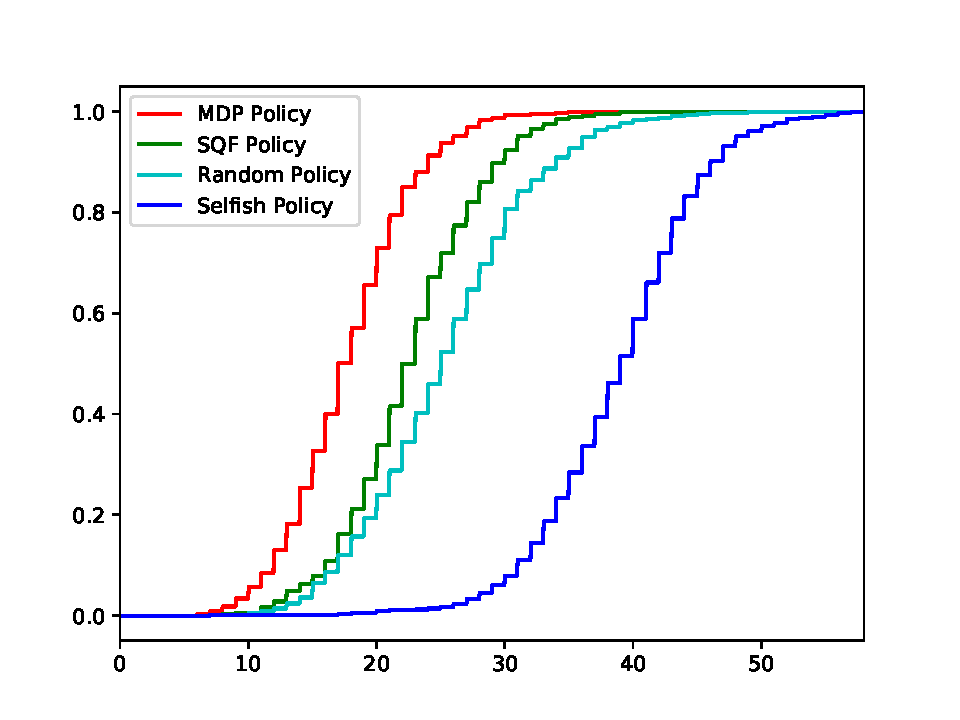
\includegraphics[width=0.30\textwidth]{images/535_LowPressure_NoDelay.pdf}&             %
        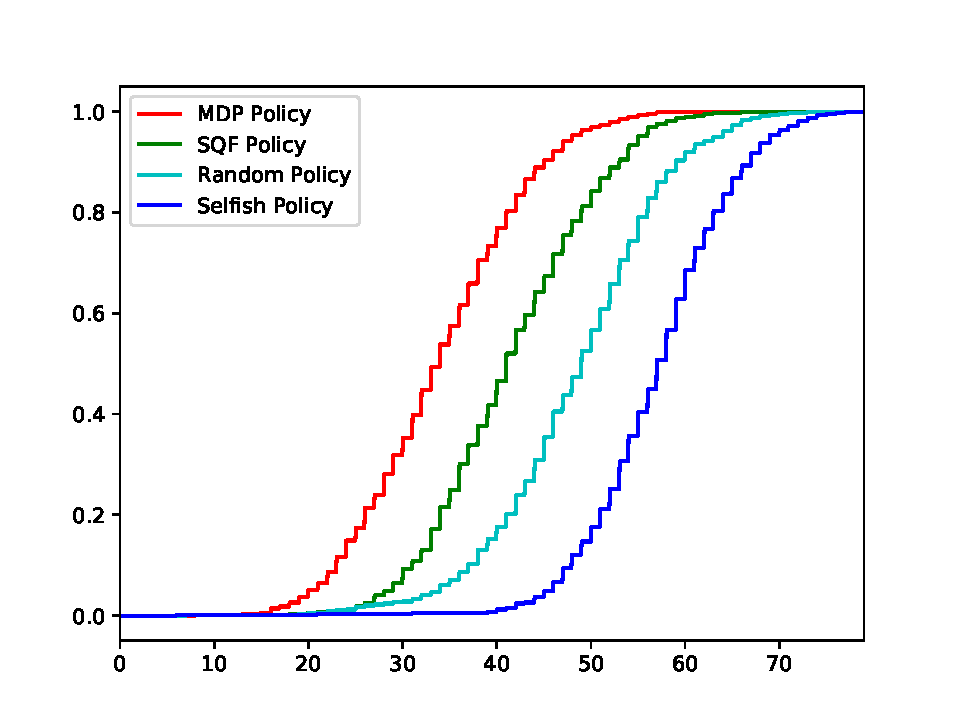
\includegraphics[width=0.30\textwidth]{images/535_LowPressure_LargeDelay_cdf.pdf}&      %
        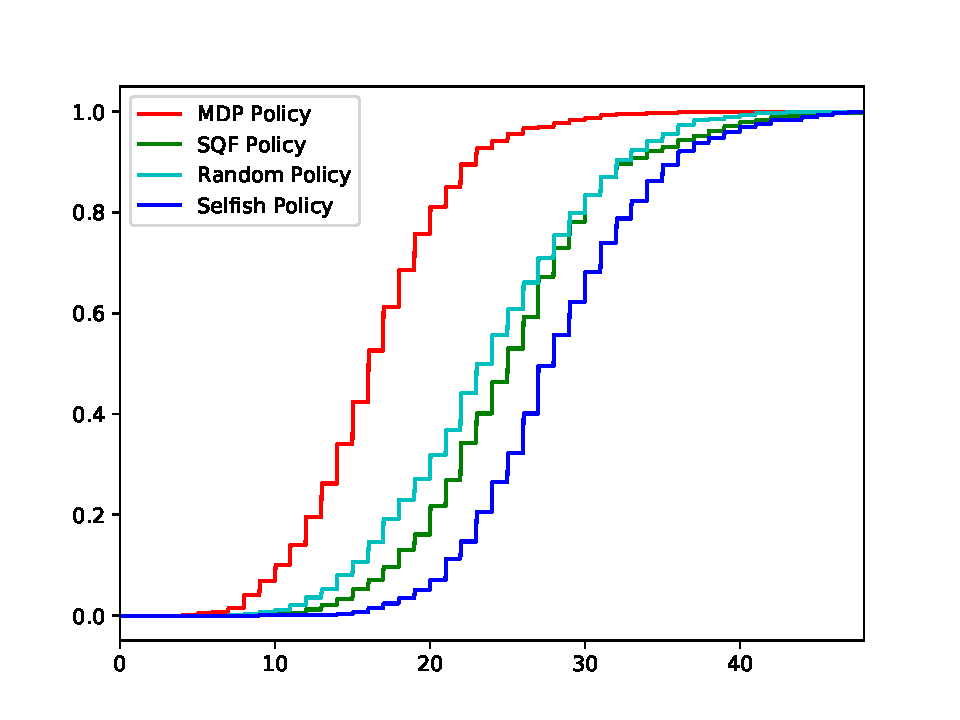
\includegraphics[width=0.30\textwidth]{images/535_LowPressure_FullDelay.pdf}            %
        \\                                                                                      %
        {\small (a) No \brlatency} &                                                            %
        {\small (b) Large \brlatency} &                                                         %
        {\small (c) Whole-interval \brlatency}                                                  %
    \end{tabular}                                                                               %
    \caption{Evaluation of Information Staleness Impact on Algorithm Robustness.}               %
    \label{fig:eval_delay}                                                                      %
\end{figure*}                                                                                   %
%-----------------------------------------------------------------------------------------------%

%-------------------------------------------------------------------%
\begin{figure}[hbt]                                                 %
    \centering                                                      %
    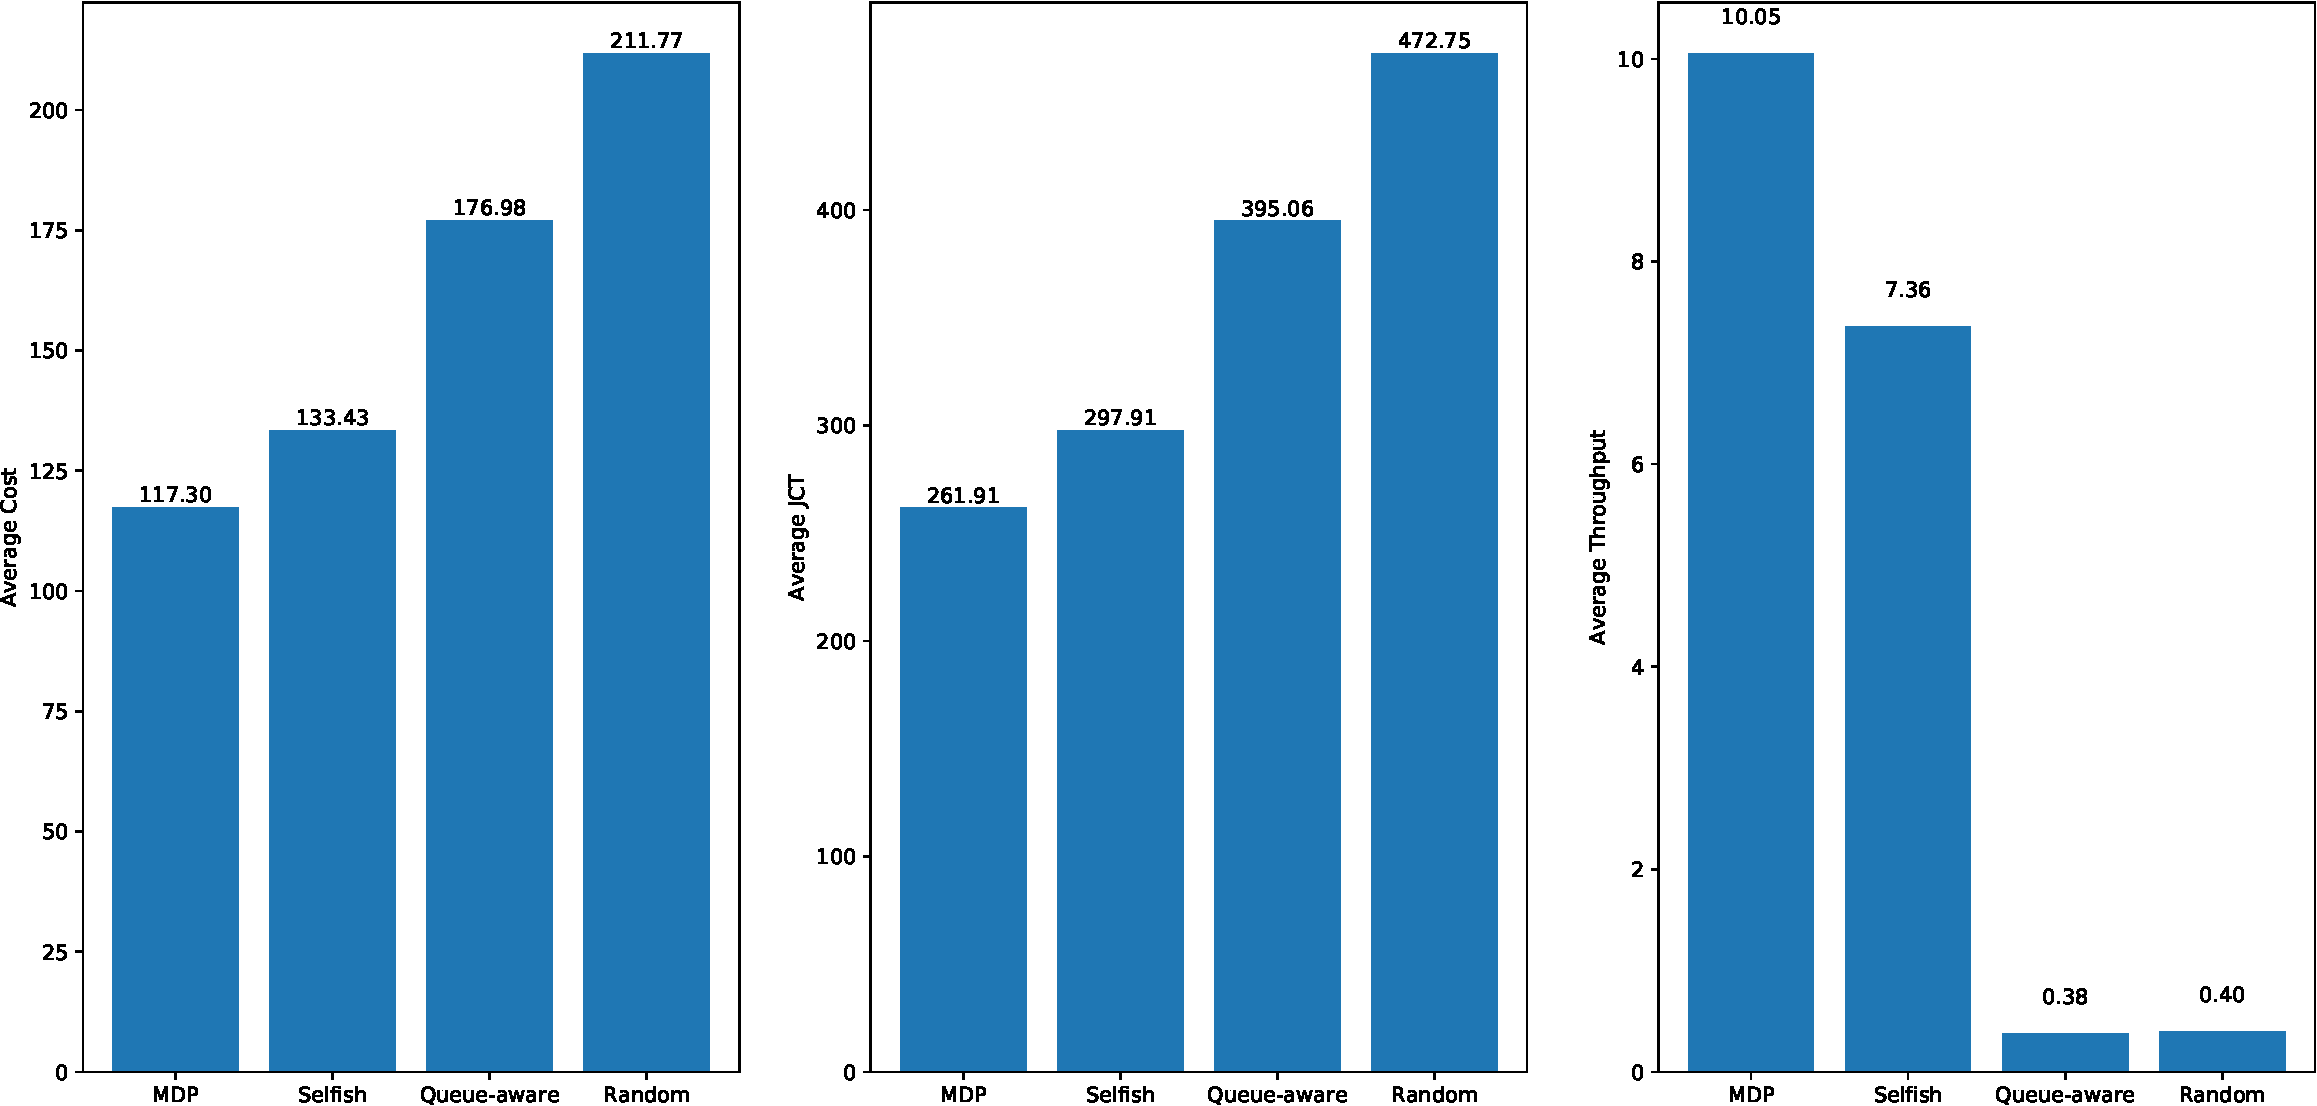
\includegraphics[width=0.45\textwidth]{bar_graph.pdf}           %
    \caption{Fake 01.}                                              %
    \label{fig:fake_01}                                             %
\end{figure}                                                        %
%-------------------------------------------------------------------%

%-------------------------------------------------------------------%
\begin{figure}[hbt]                                                 %
    \centering                                                      %
    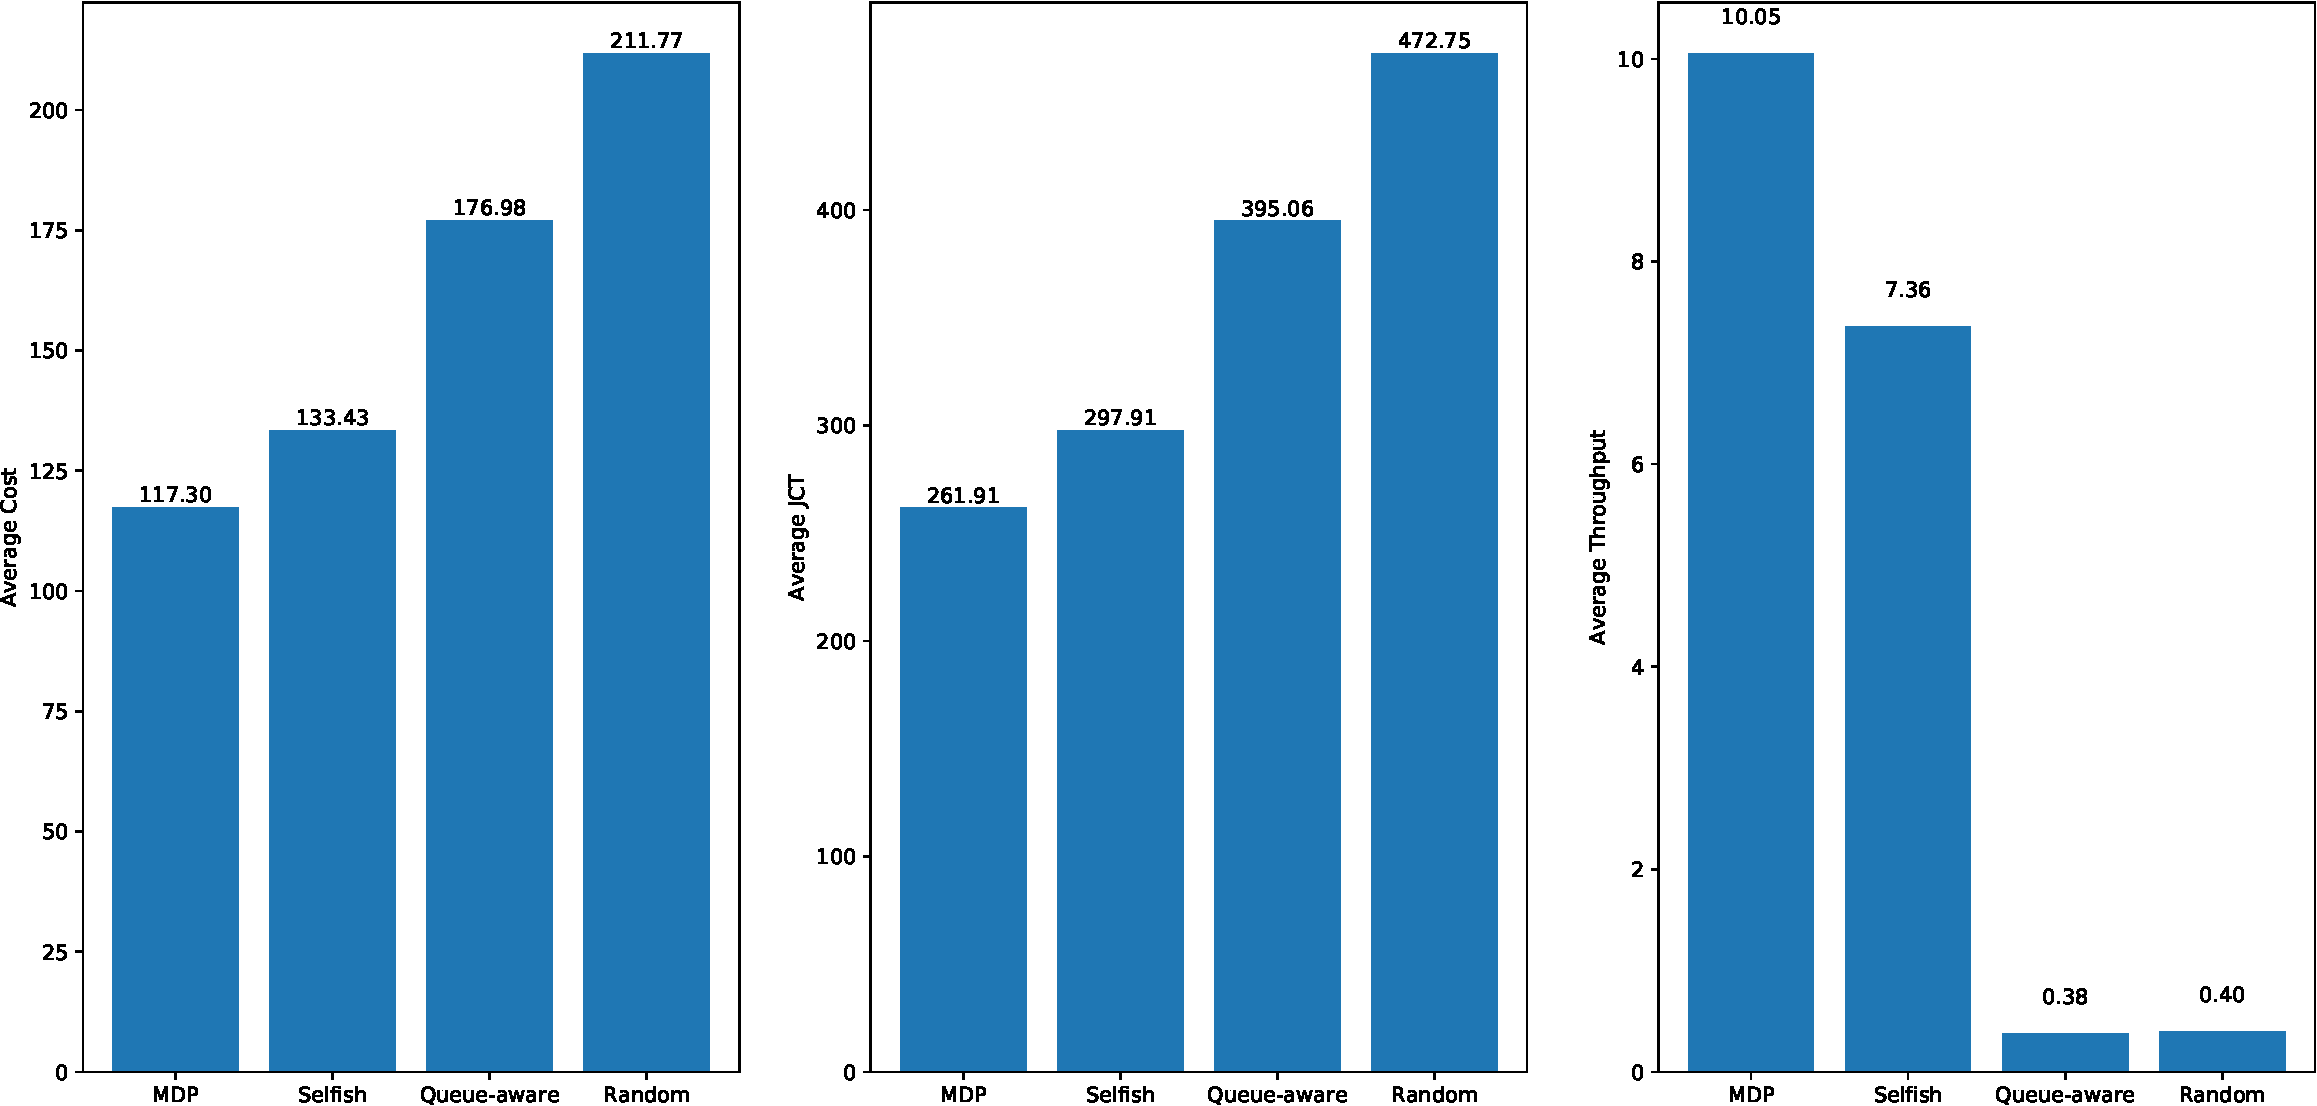
\includegraphics[width=0.45\textwidth]{bar_graph.pdf}           %
    \caption{Fake 02.}                                              %
    \label{fig:fake_02}                                             %
\end{figure}                                                        %
%-------------------------------------------------------------------%

%-------------------------------------------------------------------%
\begin{figure}[hbt]                                                 %
    \centering                                                      %
    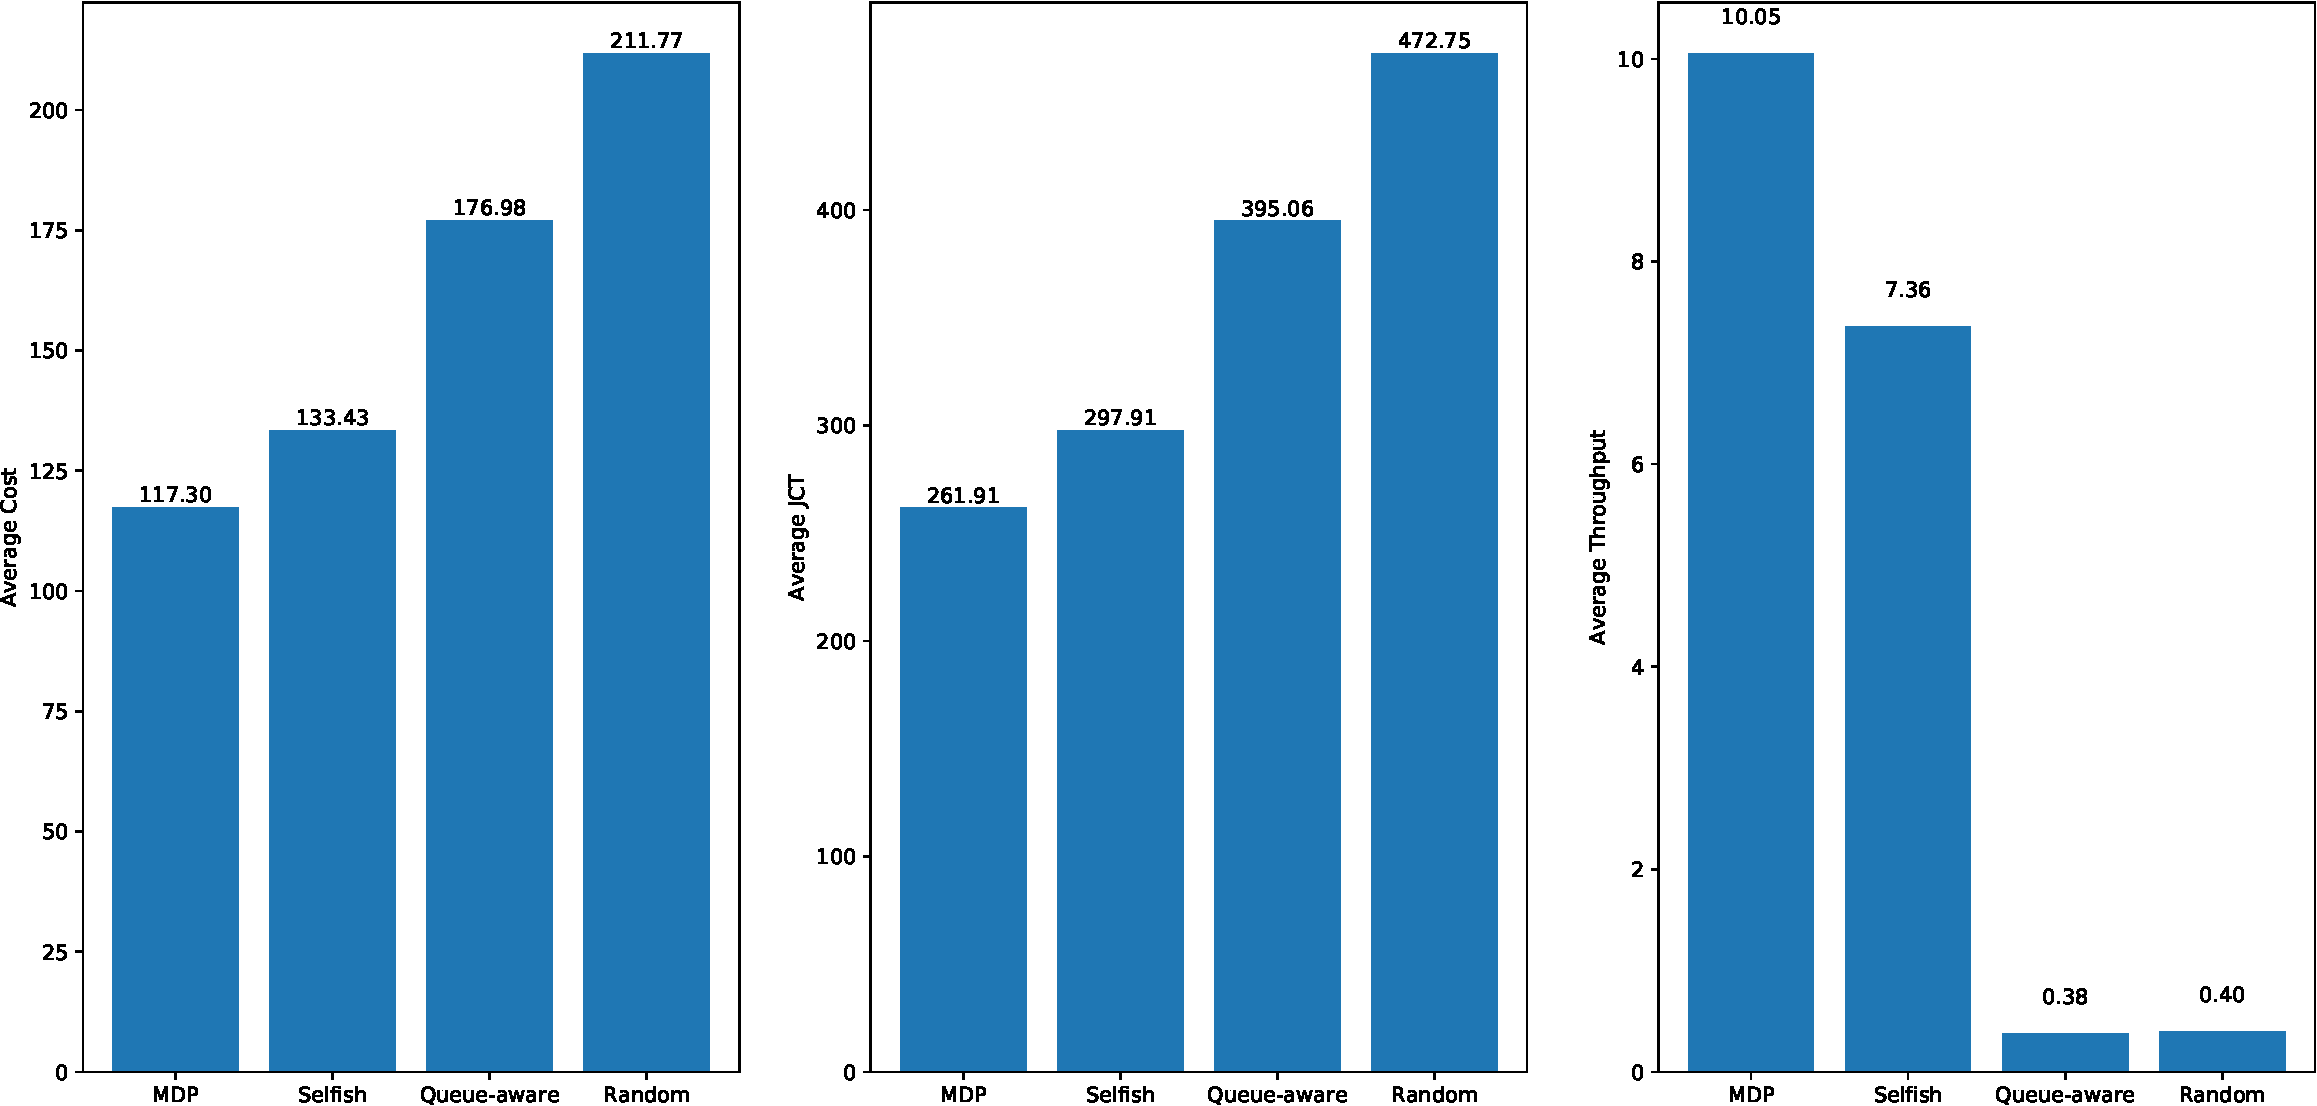
\includegraphics[width=0.45\textwidth]{bar_graph.pdf}           %
    \caption{Fake 03.}                                              %
    \label{fig:fake_03}                                             %
\end{figure}                                                        %
%-------------------------------------------------------------------%

%-------------------------------------------------------------------%
\begin{figure}[hbt]                                                 %
    \centering                                                      %
    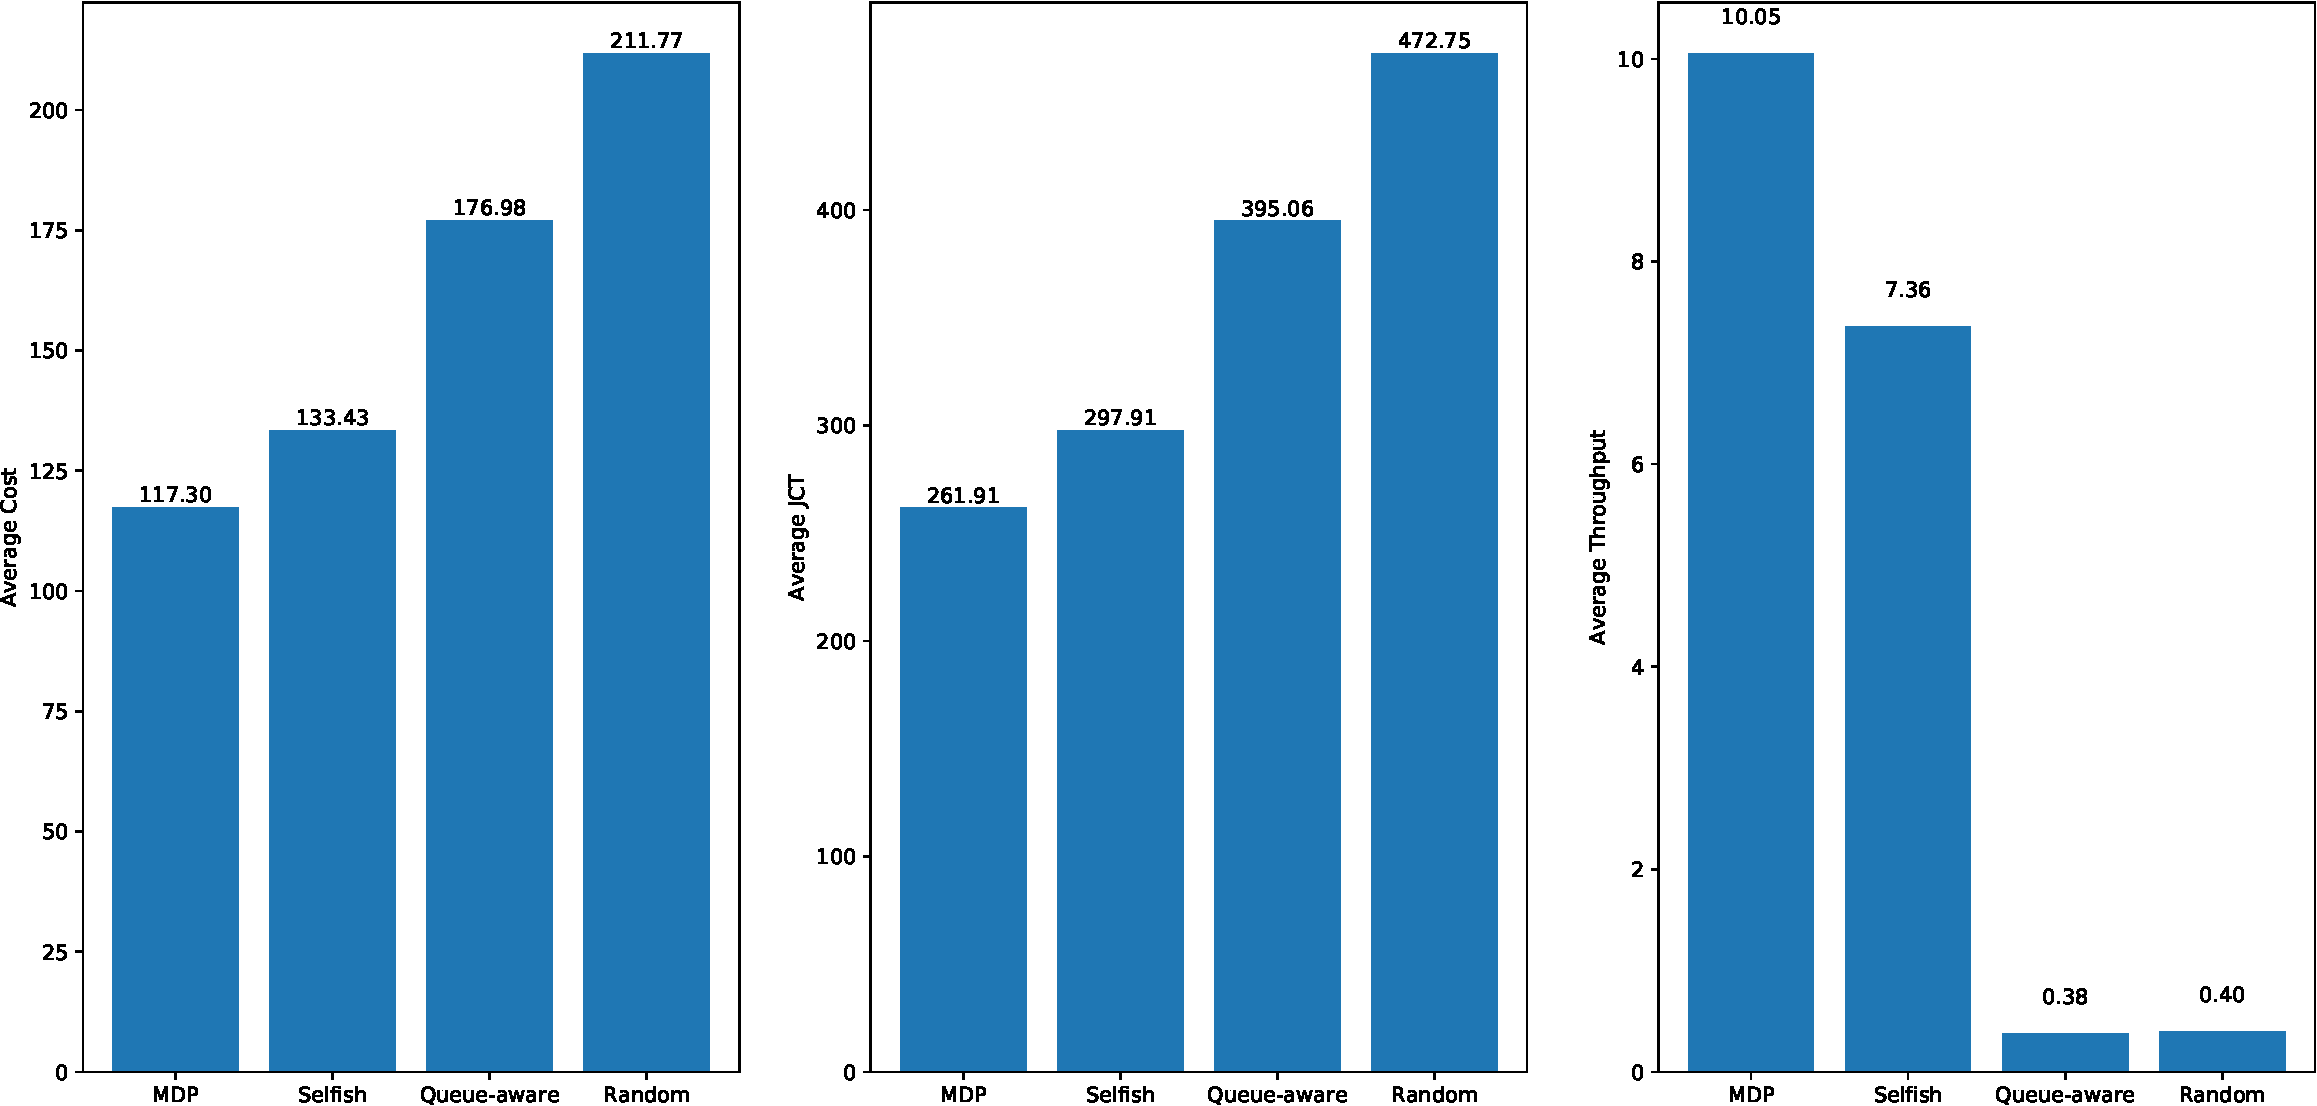
\includegraphics[width=0.45\textwidth]{bar_graph.pdf}           %
    \caption{Fake 04.}                                              %
    \label{fig:fake_04}                                             %
\end{figure}                                                        %
%-------------------------------------------------------------------%

%NOTE: 
\textbf{Compared with different \brlatency.} Fig.\ref{fig:eval_delay}
\blindtext

\textbf{Different number of APs.} (a.k.a arrival rate)
\blindtext

\textbf{Different $t_B$ setting.}
\blindtext

\textbf{Uploading time domains/Processing time domains.}
\blindtext

\textbf{Different Penalty Factors.}
\blindtext
% CDF of \# of dropped jobs (over the queue limit); CDF of queue length;
%----------------------------------------------------------------------------------------%
